\iffalse
\let\negmedspace\undefined
\let\negthickspace\undefined
\documentclass[journal,12pt,onecolumn]{IEEEtran}
\usepackage{cite}
\usepackage{amsmath,amssymb,amsfonts,amsthm}
\usepackage{algorithmic}
\usepackage{graphicx}
\usepackage{textcomp}
\usepackage{xcolor}
\usepackage{txfonts}
\usepackage{listings}
\usepackage{enumitem}
\usepackage{mathtools}
\usepackage{gensymb}
\usepackage{comment}
\usepackage[breaklinks=true]{hyperref}
\usepackage{tkz-euclide} 
\usepackage{listings}
\usepackage{gvv}                                        
\def\inputGnumericTable{}                                 
\usepackage[latin1]{inputenc}                                
\usepackage{color}                                            
\usepackage{array}                                            
\usepackage{longtable}                                       
\usepackage{calc}                                             
\usepackage{multirow}                                         
\usepackage{hhline}                                           
\usepackage{ifthen}                                           
\usepackage{lscape}
\newtheorem{theorem}{Theorem}[section]
\newtheorem{problem}{Problem}
\newtheorem{proposition}{Proposition}[section]
\newtheorem{lemma}{Lemma}[section]
\newtheorem{corollary}[theorem]{Corollary}
\newtheorem{example}{Example}[section]
\newtheorem{definition}[problem]{Definition}
\newcommand{\BEQA}{\begin{eqnarray}}
\newcommand{\EEQA}{\end{eqnarray}}
\newcommand{\define}{\stackrel{\triangle}{=}}
\theoremstyle{remark}
\newtheorem{rem}{Remark}
\begin{document}
\bibliographystyle{IEEEtran}
\vspace{3cm}
\title{NCERT 11.9.2 16Q}
\author{EE23BTECH11021 - GANNE GOPI CHANDU$^{*}$% <-this % stops a space
}
\maketitle
\bigskip
\renewcommand{\thefigure}{\theenumi}
\renewcommand{\thetable}{\theenumi}
\bibliographystyle{IEEEtran}
\textbf{Question}\\
Between 1 and 31, m numbers have been inserted in such a way that the resulting sequence is an A.P. and 
the ratio of 7 th and (m - 1) th numbers is 5:9. Find the value of m.\\
\textbf{Solution}\\
\fi
\begin{table}[!h]
\begin{center}
\renewcommand\thetable{1}
\begin{tabular}{ |c|c|c| } 
  \hline
    Symbol & Value & description \\ 
  \hline
  $x(0)$ & $1$ & First term of A.P  \\ 
  \hline
  $x(n)$ & $31$ & $\brak{n+1}\text{th}$ term \\
  \hline
  $\frac{x\brak{7}}{x\brak{m-1}}$ & $\frac{5}{9}$ & ratio of $7$ th  and $(m-1)$ th numbers\\ 
  \hline
  $n$ & $m+2$ & number of terms \\
  \hline
\end{tabular}
\end{center}
\caption{}
\end{table}\\
The last term is
\begin{align}
x(n)&=x(0)+\brak{n}d\\
\implies31 &= 1 + \brak{m + 1}d \\
\implies30 &= \brak{m + 1}d \\
\implies\frac{30}{m + 1} &= d \label{eq11.9.2.4}
\end{align}
Now $7$th and $\brak{m-1}$th terms
\begin{align}
x\brak{7} &= x(0) + 7d\label{eq11.9.2.5}\\
x\brak{m-1} &= x(0) + \brak{m-1}d\label{eq11.9.2.6}
\end{align}
From  equations \eqref{eq11.9.2.5} and \eqref{eq11.9.2.6}\\
\begin{align}
   \frac{x(0) + 7d}{x(0) + \brak{m-1}d} &= \frac{5}{9} \label{eq11.9.2.7}
\end{align}
Substituting  \eqref{eq11.9.2.4} in \eqref{eq11.9.2.7}\\
\begin{align}
\implies \frac{1+7\brak{{\frac{30}{m+1}}}}{1+\brak{{m-1}}\brak{\frac{30}{m+1}}} &= \frac{5}{9} \\
\implies \frac{m+1+210}{m+1+30m-30} &= \frac{5}{9}\\
\implies \frac{m+181}{31m-29} &= \frac{5}{9}\\
\implies 9m+1899 &=155m-145\\
\implies 155m-9m &=1899+145\\
\implies 146m &=2044\\
\implies m &=14
\end{align}
Therefore, $m = 14$ .\\
 \text{General term of AP is} \\
\begin{align}
    x\brak{n}&=\brak{2n+1}u(n)\\
    x\brak{n}&=\brak{2n}u\brak{n}+u\brak{n}
\end{align}
\begin{figure}
    \centering
    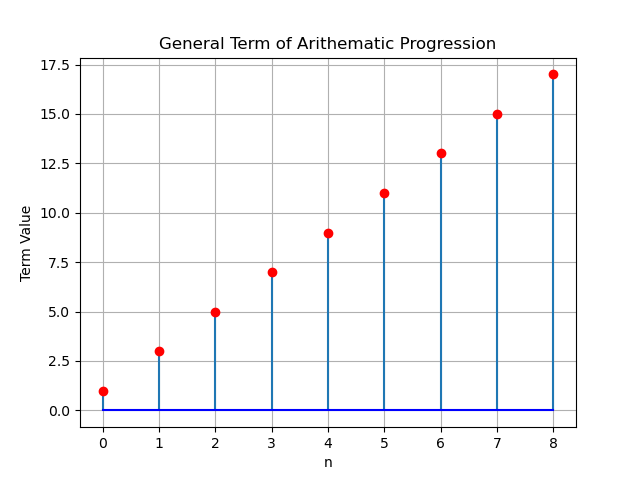
\includegraphics[width=1.0\linewidth]{ncert-maths/11/9/2/16/figs/test.png}
    \caption{Plot of x(n) vs n}
    \label{fig:11.9.2.1}
\end{figure}\\
The Z-Transform is\\
\begin{align}
    X\brak{z}&=2\brak{\dfrac{z}{\brak{z-1}^{2}}}+U\brak{z}\\
    &=\dfrac{2z}{\brak{z-1}^{2}}+\dfrac{1}{1-z^{-1}}\\
    X\brak{z}&=\dfrac{z^2+z}{\brak{z-1}^{2}} \quad{|z|>1}
\end{align}
